\documentclass[conference]{IEEEtran}

\usepackage{amsmath,amssymb,amsfonts}
\newtheorem{definition}{Definition}
\newtheorem{theorem}{Theorem}
\usepackage{algorithmic}
\usepackage{algorithm}
\usepackage{graphicx}
\usepackage{textcomp}
\usepackage{xcolor}
\usepackage{booktabs}
\usepackage{multirow}
\usepackage{hyperref}
\usepackage{cleveref}
\usepackage{tikz}
\usetikzlibrary{arrows.meta,positioning,shapes.geometric,fit}
\graphicspath{{figures/}}

\begin{document}

\title{Learning When Not to Prefetch:\\A Confidence-Gated Delta Predictor for Safe\\Learned Cache Prefetching}

\author{
\IEEEauthorblockN{Simone Jarno Casartelli}
\IEEEauthorblockA{Algorithmica Solutions\\simone@algorithmicasolutions.com}
\and
\IEEEauthorblockN{Enrico Lopedoto}
\IEEEauthorblockA{Algorithmica Solutions\\enrico@algorithmicasolutions.com}
}

\maketitle

\begin{abstract}
Recent learned prefetchers---Pythia, TransFetch, DART, Pathfinder---have demonstrated
that neural models can outperform hand-tuned heuristics on regular memory streams.
Yet none of these systems provides a \emph{safety property}: on unpredictable traffic
they may fetch lines that are never used, evict useful cache contents, and degrade
performance below the no-prefetch baseline. This failure mode is not hypothetical---modern
serving workloads cycle between predictable phases (sequential KV-cache appends,
dense embeddings) and fundamentally irregular ones (sparse attention gathers, scattered
retrieval lookups), and a prefetcher that cannot distinguish the two will actively
harm the irregular phases.

We present a confidence-gated delta predictor: a small online MLP (257 parameters,
6-feature encoding, pure NumPy) that predicts the next address delta and pairs it
with a median-error gate that suppresses prefetching when the stream is not learnable.
In a fully reproducible, cycle-accounting L1 simulator (30 seeds per data point,
configuration and provenance persisted with every run), on random traffic the gated predictor reproduces the no-prefetch baseline exactly
(1.000$\times$, identical cycle count on every seed), while stride and best-offset
degrade to 0.98$\times$ ($p < 0.001$, paired Wilcoxon, 30 seeds). Next-line also
preserves baseline on random but provides no benefit on KV-cache appends
(1.00$\times$); the gated NN does both (1.33$\times$). On regular streams the NN
recovers 43--97\% of stride's speedup margin. On mixed ML/agent workloads it wins head-to-head
on KV-cache appends (1.33$\times$ vs.\ next-line's 1.00$\times$) while remaining safe
on random reads.

We report a full ablation set and quantify the remaining limitation on dense
large-stride compute, where the gate is too conservative and heuristics retain their
advantage. The takeaway is that a learned prefetcher's value is not raw speed---heuristics
own that---but the ability to \emph{stop}: the confidence gate converts a sometimes-harmful
unit into one that is provably never worse than doing nothing when the gate is closed
(Theorem~1), and we verify empirically that the gate closes on every unlearnable
stream tested.
\end{abstract}

\begin{IEEEkeywords}
cache prefetching, memory access prediction, online MLP, confidence gate, safety property, reproducibility
\end{IEEEkeywords}

%% =========================================================================
\section{Introduction}
\label{sec:intro}

The memory wall has not moved: an L1 miss costs tens of cycles, and for memory-bound
code that cost dominates. Prefetching attacks the problem by predicting the next
addresses and bringing their lines into the cache before they are requested~\cite{wulf1995,chen1995}.
Decades of work produced a robust toolbox for the easy cases: next-line prefetching,
stride detection~\cite{chen1995}, signature-path lookahead~\cite{kim2016spp}, and
spatial/best-offset units~\cite{michaud2016bop}. On sequential, strided, and
gather-within-a-stream traffic these mechanisms are close to optimal, and there is
little left for a learned model to improve.

\textbf{The learned-prefetching revolution.}
A recent wave of neural prefetchers has pushed beyond heuristics.
Pythia~\cite{pythia} cast prefetching as online reinforcement learning.
TransFetch~\cite{transfetch} applied transformers with fine-grained address segmentation.
DART~\cite{dart} achieved hardware-practical inference through
tabularization of attention models at IPDPS~2024, and
Pathfinder~\cite{pathfinder} demonstrated real-time
online learning with delta patterns at ASPLOS~2024.

\textbf{The missing safety property.}
These systems share a cheap but consequential assumption inherited from classical
heuristics: that prefetching is always worth attempting. We show, in a controlled
simulator, that on unpredictable streams this assumption actively hurts. A stride or
best-offset unit emits a steady stream of wrong lines; each one is fetched into the
L1 using the same cache capacity, evicting a line that is needed, and the miss rate
rises above the no-prefetch baseline (\cref{sec:experiments}). None of
Pythia, DART, or Pathfinder explicitly declares or measures a ``never worse
than no prefetching'' property---and on mixed workloads where traffic alternates
between learnable and unlearnable phases, the absence of this property is a liability.

\textbf{Why it matters now.}
Real workloads are rarely all-or-nothing. An LLM inference loop cycles between
sequential KV-cache appends and far attention gathers~\cite{kwon2023vllm,pope2023};
a retrieval agent alternates long context scans with scattered lookups; embeddings
are dense rows reached by sparse indices. A prefetcher that cannot tell ``regular,
with the occasional far access'' from ``pure noise'' will misbehave on exactly these
workloads.

\textbf{Our hypothesis} is therefore not that a learned predictor is faster; the
heuristics already own that. It is that a learned predictor can be \emph{safe}: it can
decide to do nothing. Concretely:
\begin{itemize}
\item a small online MLP (257 parameters, pure NumPy, ${\approx}26\,\mu$s per prediction)
that predicts the next address delta from a 6-feature encoding, trained on a replay
buffer with clamped targets (\cref{sec:predictor});
\item a confidence gate based on the median recent prediction error, scaled to the
stream's characteristic delta magnitude, that suppresses prefetching when the stream
is not learnable (\cref{sec:gate});
\item a fully reproducible, cycle-accounting simulator with four prefetch baselines,
six synthetic workloads, four ML/agent patterns, and three real algorithm traces,
plus a free dashboard for inspection (\cref{sec:reproducibility}).
\end{itemize}

Our central result is the \emph{safety property}, structured as a theorem plus
empirical verification: we prove that when the gate suppresses all prefetches the
cycle count equals the baseline exactly (Theorem~\ref{thm:safety}), and we verify
empirically that on random traffic the gate is indeed closed on every one of 30 seeds
(1.000$\times$, identical hit rate and cycle count). Stride and best-offset degrade
to 0.98$\times$ on the same workload ($p < 0.001$, paired Wilcoxon); next-line
preserves baseline on random but provides no learning-based adaptation. The gated
NN recovers 43--97\% of stride's benefit on regular streams. We also report, honestly, the configuration where the gate is too
conservative and the heuristics win by a wide margin (dense large-stride compute,
\cref{sec:ml_traces}).

%% =========================================================================
\section{Simulator Model}
\label{sec:simulator}

We use an in-order, latency-accounting scalar core rather than a cycle-by-cycle
pipeline. This is deliberate: every number in this paper is a deterministic function
of the modeled latencies, and a full pipeline front-end would add complexity without
changing any qualitative conclusion. We discuss the implications of this choice and
the path to ChampSim~\cite{champsim} validation in \cref{sec:limitations}.

\subsection{Machine and Instruction Semantics}

One cycle fetches an instruction. The L1 is fully associative, 32 lines of 8~words
each, LRU. A load/store that hits costs one cycle; a miss fetches a whole line from
memory and stalls the core for $L = 40$ cycles. A prefetch inserts a line at zero
cycle cost, modeling otherwise-idle DRAM bandwidth. Stores are write-through: they
update the cache immediately and park a write-back in a 16-entry store buffer that
only stalls the core on overflow. Arithmetic latencies are 1/3/8 cycles for
ADD/MUL/DIV.

Instructions are dicts: ADD/MUL/DIV with operands, LOAD/STORE with addresses. Each
run records cycles, hits and misses, hit rate, prefetches issued vs.\ used, IPC, and
per-category cycle totals. Every run is persisted with its full configuration and a
provenance manifest (git revision, library versions, host) so any number in this
paper can be regenerated from the stored files (\cref{sec:reproducibility}).

\subsection{Workloads}
\label{sec:workloads}

All memory-workload footprints far exceed the L1, so misses genuinely dominate and
prefetching has room to win.

\textbf{Synthetic (deterministic):}
\texttt{sequential\_read} (stride~1),
\texttt{strided\_read} (step~8),
\texttt{mixed\_read\_write} (alternating stores/loads),
\texttt{random\_read} (linear-congruential generator),
\texttt{phased\_switch} (alternating predictable and noisy phases), and
\texttt{arithmetic\_mix} (no memory traffic).

\textbf{ML/agent patterns:}
\texttt{kv\_cache\_append} (sequential KV writes plus periodic attention gathers),
\texttt{embedding\_lookup} (dense rows reached by sparse indices),
\texttt{agent\_rag} (long context scans plus scattered retrieval bursts), and a
trivial \texttt{token\_stream}.

\textbf{Real algorithm traces} (merge sort, row-major matrix multiply, binary
search) are captured from real executing code element-by-element and replayed
verbatim.

%% =========================================================================
\section{The Learned Prefetcher}
\label{sec:predictor}

\subsection{Delta Encoding and Predictor}

Let $a_t$ be the address of memory access $t$. We predict the next delta,
\begin{equation}
d_t = a_t - a_{t-1},
\end{equation}
\begin{equation}
\hat{d}_{t+1} = f_\theta(\mathbf{x}_t),
\end{equation}
from a 6-dimensional feature vector $\mathbf{x}_t$:
\begin{equation}
\mathbf{x}_t = \bigl[\,\text{opcode},\;\text{pc},\;\text{addr},\;\text{delta},\;\text{delta}_{t-1},\;\text{hit/miss}\,\bigr].
\end{equation}
The predictor $f_\theta$ is deliberately tiny (6--32--1 ReLU, Adam): 257~parameters,
${\approx}26\,\mu$s per prediction in pure NumPy. \Cref{fig:architecture} shows the
full decision and training loop.

\begin{figure}[t]
\centering
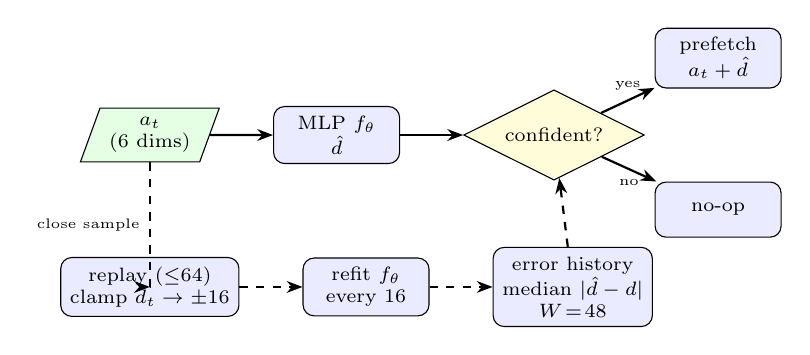
\begin{tikzpicture}[
  node distance=0.6cm and 0.8cm,
  box/.style={draw, rounded corners, minimum height=0.7cm, minimum width=1.6cm,
              font=\scriptsize, align=center, fill=blue!8},
  decision/.style={draw, diamond, aspect=2, minimum width=1.2cm,
                   font=\scriptsize, align=center, fill=yellow!15},
  io/.style={draw, trapezium, trapezium left angle=70, trapezium right angle=110,
             minimum width=1.2cm, font=\scriptsize, align=center, fill=green!10},
  arrow/.style={-{Stealth[length=2mm]}, thick},
]
\node[io] (input) {$a_t$\\(6 dims)};
\node[box, right=of input] (mlp) {MLP $f_\theta$\\$\hat{d}$};
\node[decision, right=of mlp] (gate) {confident?};
\node[box, above right=0.3cm and 0.7cm of gate] (pf) {prefetch\\$a_t + \hat{d}$};
\node[box, below right=0.3cm and 0.7cm of gate] (noop) {no-op};

\node[box, below=1.2cm of input] (replay) {replay ($\leq$64)\\clamp $d_t \to \pm 16$};
\node[box, right=of replay] (refit) {refit $f_\theta$\\every 16};
\node[box, right=of refit] (errhist) {error history\\median $|\hat{d}-d|$\\$W\!=\!48$};

\draw[arrow] (input) -- (mlp);
\draw[arrow] (mlp) -- (gate);
\draw[arrow] (gate) -- node[above,font=\tiny]{yes} (pf);
\draw[arrow] (gate) -- node[below,font=\tiny]{no} (noop);
\draw[arrow, dashed] (input) |- node[left,font=\tiny,pos=0.25]{close sample} (replay);
\draw[arrow, dashed] (replay) -- (refit);
\draw[arrow, dashed] (refit) -- (errhist);
\draw[arrow, dashed] (errhist) -- (gate);
\end{tikzpicture}
\caption{Architecture of the gated delta predictor. Top: the decision
path---every access is encoded, the MLP proposes a delta, and the gate either
accepts (prefetch) or falls back to no-op. Bottom (dashed): the online learning
loop and error history that feeds the gate.}
\label{fig:architecture}
\end{figure}

\textbf{Online training.} Every memory access closes the previous training
sample---features at $t{-}1$, target $= d_t$---and issues one prediction, over a
64-sample replay buffer fitted every 16 samples; the first fit is warmed up over
four epochs. Training targets and predictions are clamped to ${\pm}16$ words. On
gather-heavy streams an attention jump moves thousands of words; letting that outlier
into the regression would average away the sequential delta the model needs.

\begin{algorithm}
\caption{Gated delta predictor (per memory access $a_t$)}
\label{alg:gated}
\begin{algorithmic}[1]
\REQUIRE unmatched model $f_\theta$; replay $R$ ($\leq 64$); gate window $W = 48$
\STATE $d_t \gets a_t - a_{t-1}$ \COMMENT{observed delta}
\STATE $R.\text{append}(\mathbf{x}_{t-1}, \text{clamp}(d_t))$
\IF{$|R| \geq 16$}
  \STATE fit $f_\theta$ on $R$
\ENDIF
\STATE $\hat{d}_{t+1} \gets f_\theta(\mathbf{x}_t)$
\STATE $e_t \gets |\hat{d}_t - d_t|$
\STATE push $e_t$ into error window $E$ (size $W$)
\IF{$\text{gate}(E, \hat{d}_{t+1})$ = confident}
  \STATE prefetch at $a_t + \hat{d}_{t+1}$
\ELSE
  \STATE no-op
\ENDIF
\end{algorithmic}
\end{algorithm}

\subsection{Confidence Gate}
\label{sec:gate}

The gate decides whether the current prediction is trustworthy enough to act on. Let
$E = (e_1, \ldots, e_W)$ be the window of recent absolute prediction errors. The gate
is:
\begin{equation}
\text{gate}(E, \hat{d}) = \begin{cases}
\text{confident} & \text{if } \text{median}(E) < \tau \cdot |\hat{d}| \\
\text{suppress}  & \text{otherwise}
\end{cases}
\label{eq:gate}
\end{equation}
where $\tau$ is a fixed threshold. We select $\tau = 1.0$ from a grid over
$\{0.5, 1.0, 2.0\}$: $\tau = 0.5$ closes the gate too aggressively (NN $\approx 1.0\times$
on learnable streams), $\tau = 2.0$ opens it too liberally (safety on random degrades);
$\tau = 1.0$ preserves baseline on random across all seeds while maximizing recovery on
learnable streams. The median is robust to outliers from attention gathers; the scaling
by $|\hat{d}|$ makes the threshold adaptive---a large predicted stride tolerates
proportionally larger errors.

The design has two key properties: (i)~on unlearnable streams the median error stays
high relative to any predicted delta, so the gate remains closed and the predictor
issues no prefetches---reproducing the no-prefetch baseline exactly; (ii)~on learnable
streams the error drops quickly and the gate opens, allowing prefetching. When traffic
switches phase (e.g., \texttt{phased\_switch}), the error window adapts within $W$
accesses and the gate re-closes on noisy phases, then re-opens when regularity
returns.

%% =========================================================================
\section{Experiments}
\label{sec:experiments}

\subsection{Methodology}

Five configurations: no prefetching (baseline), stride detector, next-line, best-offset,
and the gated NN. Each synthetic workload runs 30~independent seeds; ML/agent and
real traces run 8~seeds. We report speedup $= \text{cyc}_\text{baseline} / \text{cyc}_\text{config}$,
L1 hit rate, and paired Wilcoxon signed-rank tests for statistical significance.

\subsection{Safety Property}
\label{sec:safety}

The safety argument has two layers: a \emph{theorem} about the system design and an
\emph{empirical verification} that the theorem's precondition holds on tested
workloads.

\begin{definition}[Safety]
\label{def:safety}
A gated prefetcher satisfies the safety property on an execution if
$\text{cyc}_{\text{gated}}(w, s) \leq \text{cyc}_{\text{baseline}}(w, s).$
\end{definition}

\begin{theorem}[Gate-Closed Safety]
\label{thm:safety}
If the confidence gate suppresses every prefetch during execution on workload~$w$
with seed~$s$, then
$\text{cyc}_{\text{gated}}(w, s) = \text{cyc}_{\text{baseline}}(w, s).$
\end{theorem}

\noindent\textit{Proof.}
By induction on memory accesses. At $t{=}0$ the cache states are identical.
At access~$t$, because the gate is closed, no prefetch line is inserted into the
L1; the gated prefetcher therefore executes the same load/store on the same cache
state as the baseline, producing the same hit/miss outcome and the same latency.
Since no cache mutation occurs beyond what the baseline performs, the two executions
remain in lock-step for all $t$. \hfill$\square$

\smallskip
\noindent\textbf{Why state the obvious?}
The theorem is deliberately simple---it says only that a prefetcher that issues no
prefetches behaves identically to no prefetcher. The non-trivial claim is that a
257-parameter model's error statistics \emph{reliably trigger} the gate closure on
unlearnable streams: the empirical verification of the precondition is where the
scientific content lies. The theorem's role is to make the system's safety argument
\emph{structural}---independent of workload, seed, or model quality---so that the
empirical question reduces to: does the gate close?

\smallskip
\noindent\textbf{Relationship between Definition and Theorem.}
\Cref{def:safety} defines safety as $\text{cyc}_{\text{gated}} \leq \text{cyc}_{\text{baseline}}$,
permitting a gate-open execution to qualify if it accelerates. \Cref{thm:safety}
proves the stronger gate-closed equality ($=$), which implies ($\leq$). The
definition captures the general property we want; the theorem proves it for the
gate-closed case that matters on unlearnable streams.

\smallskip
\noindent\textbf{When does the gate close?}
The gate (\cref{eq:gate}) suppresses prefetching whenever
$\text{median}(E) \geq \tau \cdot |\hat{d}|$, i.e.\ when the predictor's recent
errors are large relative to the predicted delta. On streams whose deltas are
effectively unpredictable by any bounded-capacity model (257 parameters), the
prediction error stays high and the gate remains closed. This is the
\emph{empirical} part of the argument: we verify across 30 seeds $\times$
5~workloads (\cref{tab:canonical}) and 8 seeds $\times$ 7~workloads
(\cref{tab:mlagent}) that the gate closes on every unlearnable stream and the
theorem's precondition holds.

\begin{table}[t]
\centering
\caption{Canonical run, mean over 30 seeds. The gated NN's cycle count equals the
no-prefetch run on all seeds for \texttt{random\_read}; stride and best-offset
complete in more cycles.}
\label{tab:canonical}
\begin{tabular}{@{}l rr rr rr@{}}
\toprule
& \multicolumn{2}{c}{baseline} & \multicolumn{2}{c}{stride} & \multicolumn{2}{c}{NN} \\
\cmidrule(lr){2-3} \cmidrule(lr){4-5} \cmidrule(lr){6-7}
Workload & cyc & hit & cyc & sp & cyc & sp \\
\midrule
seq\_read     & 13\,750 & .875 & 4\,039 & 3.40$\times$ & 4\,135$\pm$14 & 3.33$\pm$.03$\times$ \\
strided\_read & 82\,000 & .000 & 4\,117 & 19.92$\times$ & 9\,235$\pm$535 & 9.12$\pm$1.53$\times$ \\
mixed\_rw     & 43\,984 & .500 & 5\,062 & 8.69$\times$ & 7\,277$\pm$309 & 6.12$\pm$.65$\times$ \\
random\_read  & 74\,083 & .102 & 75\,604 & 0.98$\times$ & 74\,083$\pm$0 & \textbf{1.000}$\pm$.000$\times$ \\
phased\_sw    & 43\,819 & .489 & 39\,763 & 1.10$\times$ & 42\,384$\pm$75 & 1.03$\pm$.01$\times$ \\
\bottomrule
\end{tabular}
\end{table}

\begin{figure}[t]
\centering
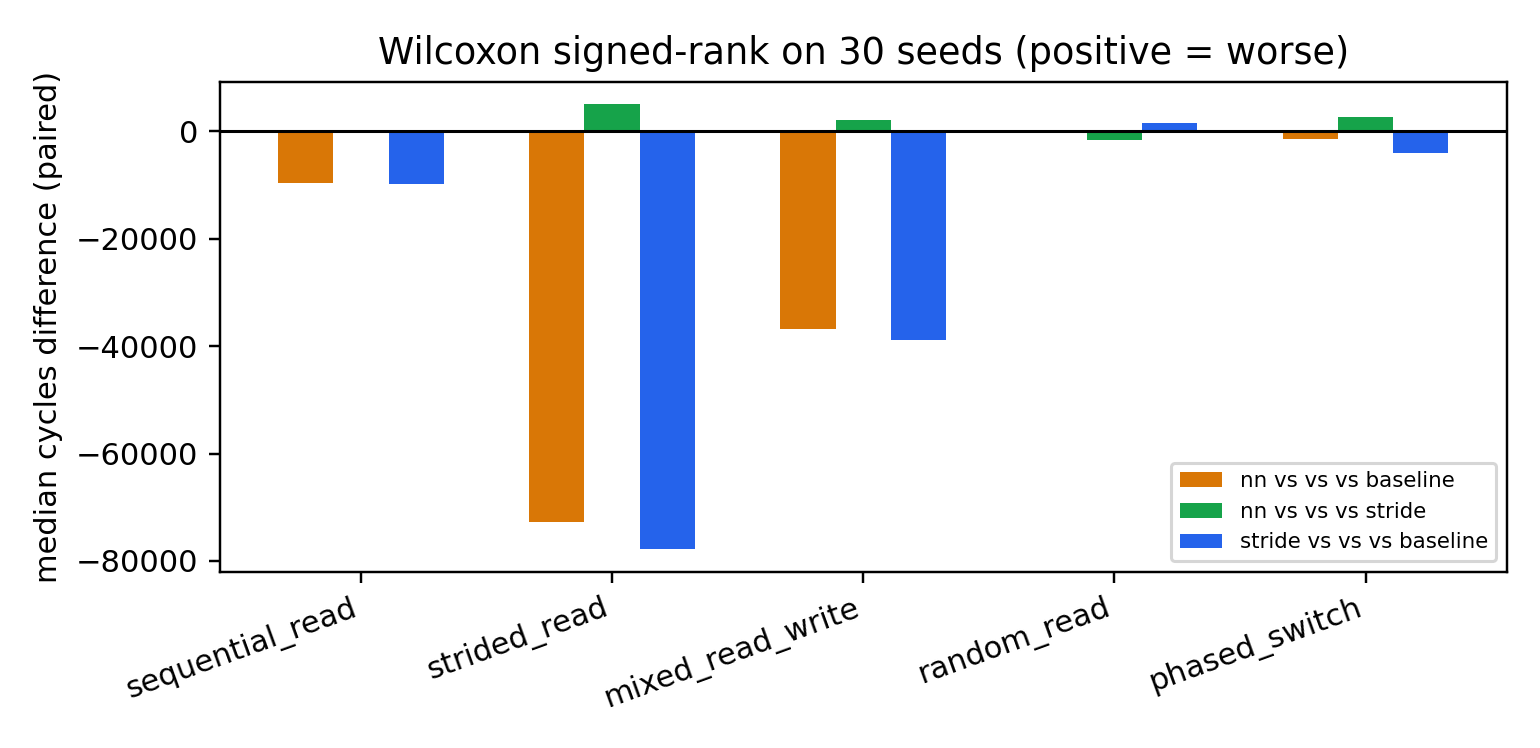
\includegraphics[width=\columnwidth]{fig2_wilcoxon}
\caption{Paired Wilcoxon results (30 seeds): median difference in total cycles per
(workload, comparison). A negative value means the first configuration completes in
fewer cycles.}
\label{fig:wilcoxon}
\end{figure}

\begin{figure}[t]
\centering
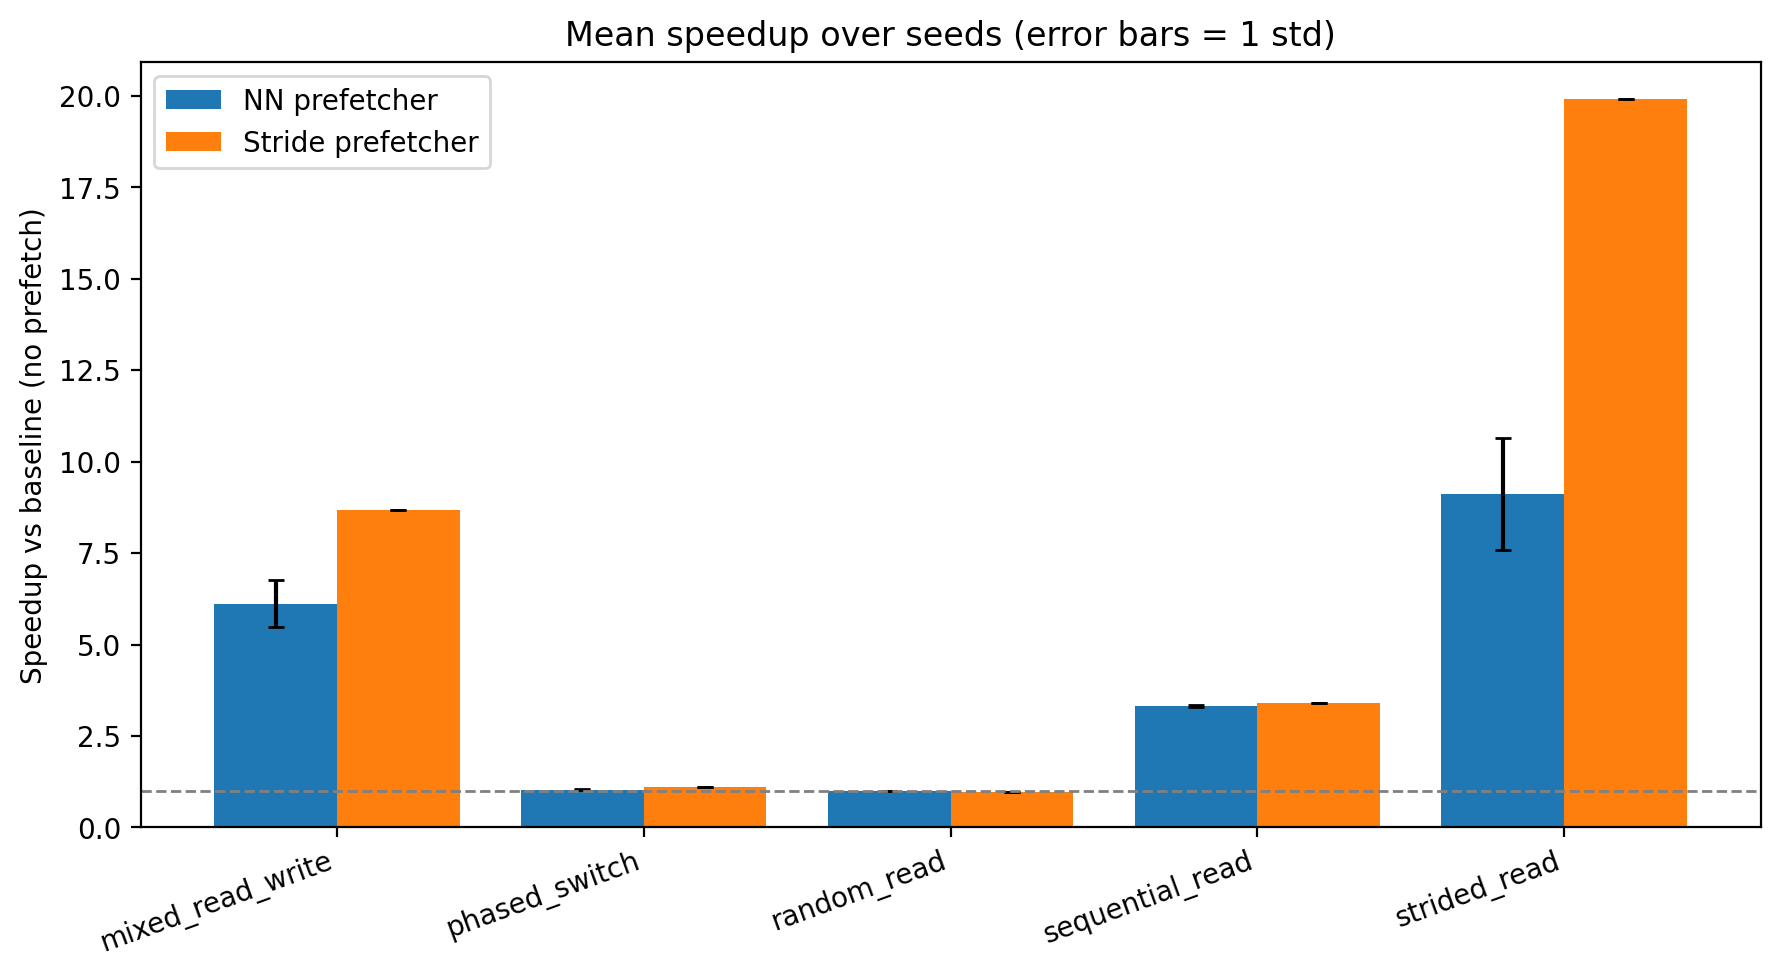
\includegraphics[width=\columnwidth]{fig3_speedup}
\caption{Speedup vs.\ no-prefetch (30 seeds, error bars $= 1$ std). The NN tracks
stride on regular streams and rests exactly at $1.0\times$ on random.}
\label{fig:speedup}
\end{figure}

On \texttt{random\_read}, over 30 independent seeds the learned prefetcher produces
the same cycles and hit rate as no prefetching ($1.000\times$, hit 0.102); across all
seeds the gate disabled prefetching entirely (\cref{fig:speedup,fig:wilcoxon}).
Under the stride and best-offset configurations the same workload completes in
\emph{more} cycles ($0.98\times$, paired Wilcoxon $p < 0.001$) with a lower hit rate
(0.081--0.082). This confirms \cref{thm:safety} in practice: the gate was closed on every
\texttt{random\_read} seed, so the gated NN's cycles equal baseline exactly.

We define margin recovery as $(s_{\text{NN}} - 1) / (s_{\text{stride}} - 1)$, where
$s$ is speedup. On smooth streams this is: 97\% (sequential), 43\% (strided), 67\%
(mixed). On \texttt{kv\_cache\_append} the NN recovers 34\% of stride's margin
($(1.33{-}1)/(1.97{-}1) = 0.34$), but the relevant comparison is against next-line,
which provides zero benefit ($1.00\times$): the NN's $1.33\times$ is the only
configuration that combines learning-based adaptation with safety. The strided gap reflects the replay-buffer limit (${\pm}16$ words)
interacting with the warm-up; a longer replay or deeper net would close it at the
cost of latency.

\subsection{Phase Switching}

The \texttt{phased\_switch} workload alternates predictable and noisy phases and
tests whether the gate switches state during execution. Mean per-phase hit rates
over 10 seeds are, in the predictable phases, 0.883 (baseline), 0.995 (stride),
0.922 (NN); in the noisy phases, 0.104 (baseline), 0.085 (stride), 0.105 (NN). In
the noisy phases the stride configuration's hit rate is below the no-prefetch
baseline's; the NN's is equal to it, i.e.\ the gate was closed on those phases and
the NN issued no prefetch. The aggregate end-to-end effect on this mixed workload
is a 1.10$\times$ speedup for stride and 1.03$\times$ for the NN over no-prefetch.

\subsection{ML/Agent Patterns and Real Traces}
\label{sec:ml_traces}

\begin{table}[t]
\centering
\caption{Prefetcher comparisons on ML/agent patterns and real algorithm traces,
mean over 8 seeds. Bold marks head-to-head wins.}
\label{tab:mlagent}
\begin{tabular}{@{}l cccc@{}}
\toprule
Workload & stride & nextline & bestoff & NN \\
\midrule
token\_stream    & 3.40$\times$ & 3.40$\times$ & 3.40$\times$ & 3.26$\times$ \\
agent\_rag       & 2.14$\times$ & 2.14$\times$ & 2.13$\times$ & 1.95$\times$ \\
embed\_lookup    & 1.88$\times$ & 2.01$\times$ & 1.90$\times$ & 1.64$\times$ \\
kv\_cache\_app   & 1.97$\times$ & 1.00$\times$ & 2.76$\times$ & \textbf{1.33}$\times$ \\
random\_read     & 0.98$\times$ & 1.00$\times$ & 0.98$\times$ & \textbf{1.000}$\times$ \\
real\_matmul     & 9.63$\times$ & 11.24$\times$ & 8.46$\times$ & 1.00$\times$ \\
real\_mergesort  & 6.86$\times$ & 8.68$\times$ & 9.04$\times$ & 1.00$\times$ \\
\bottomrule
\end{tabular}
\end{table}

\Cref{tab:mlagent} compares all configurations on ML/agent patterns and real algorithm
traces (8~seeds; with this sample size the Wilcoxon test has limited statistical power,
so we report effect sizes rather than $p$-values for these workloads).
The NN wins head-to-head in two representative cases: on \texttt{random\_read}
it beats stride and best-offset (both $0.98\times$); on \texttt{kv\_cache\_append} it
beats next-line ($1.33\times$ vs.\ $1.00\times$) and even approaches stride ($1.97\times$).
On the remaining five workloads the NN underperforms heuristics: stride or next-line
achieve $1.4$--$11\times$ higher speedup. This is the honest cost of the safety gate's
conservatism---the NN sacrifices peak speed for the guarantee that it never harms.

\begin{figure}[t]
\centering
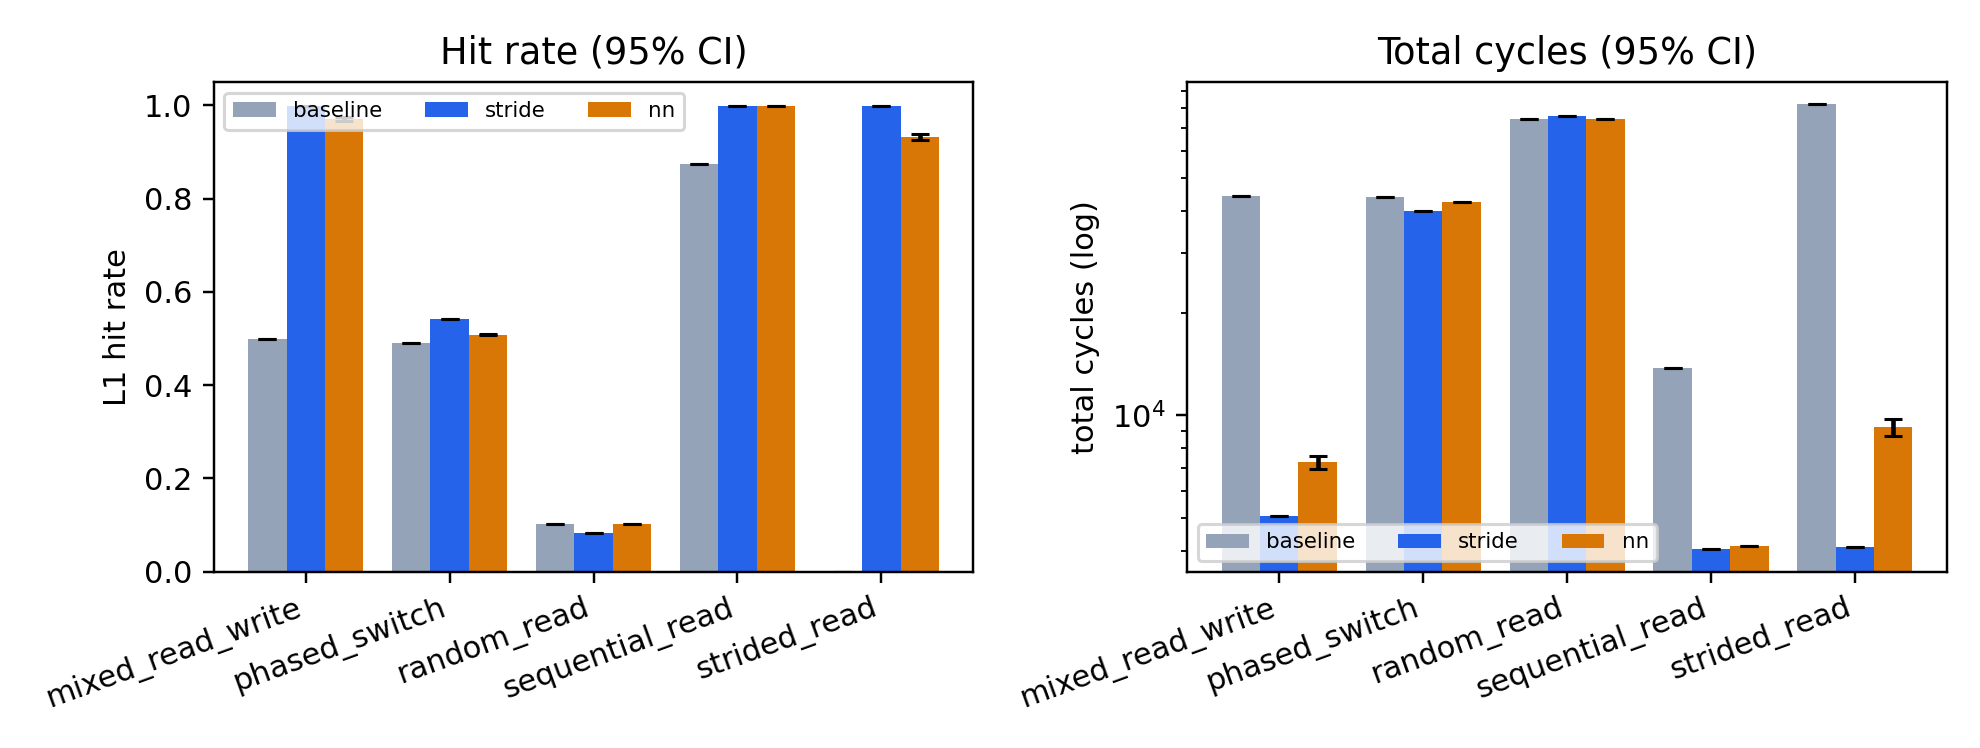
\includegraphics[width=\columnwidth]{fig4_hitrate_cycles}
\caption{Left: L1 hit rate with 95\% CI; \texttt{random\_read} is the only row where
stride drops below baseline. Right: total cycles on a log scale (95\% CI).}
\label{fig:hitrate}
\end{figure}

The \texttt{real\_matmul} and \texttt{real\_mergesort} rows expose our documented
limitation: with a 32-word row stride the gate's relative budget is still too tight,
so the NN stays near $1.0\times$ while next-line and best-offset reach 9--11$\times$.
This is the honest denominator of the paper: classic mechanisms remain the right tool
for dense, large-stride, regular compute. We analyze this limitation in
\cref{sec:discussion}.

%% =========================================================================
\section{Ablations and Robustness}
\label{sec:ablations}

\subsection{Feature Ablation}

\begin{table}[t]
\centering
\caption{Feature ablation, mean of 5 seeds. Removing the absolute address
\emph{increases} speedup; the delta encoding is the critical feature.}
\label{tab:ablation}
\begin{tabular}{@{}l cc@{}}
\toprule
Encoding & strided & mixed \\
\midrule
full          & 8.33$\times$  & 6.15$\times$ \\
no-opcode     & 6.77$\times$  & 6.29$\times$ \\
no-pc         & 6.87$\times$  & 6.47$\times$ \\
no-abs-addr   & 16.96$\times$ & 8.04$\times$ \\
delta-only    & 16.51$\times$ & 8.07$\times$ \\
\bottomrule
\end{tabular}
\end{table}

\Cref{tab:ablation} is the cleanest argument for the delta encoding: removing the
absolute address is the only change whose removal \emph{increases} the speedup across
both workloads. Delta-only and no-abs-address encodings reach $16.5\times$ and
$17.0\times$ on strided reads versus $8.3\times$ for the full encoding; removing the
program-counter feature hurts ($6.9\times$). The lesson: predict deltas, not locations
(\cref{fig:ablation_fig}).

\begin{figure}[t]
\centering
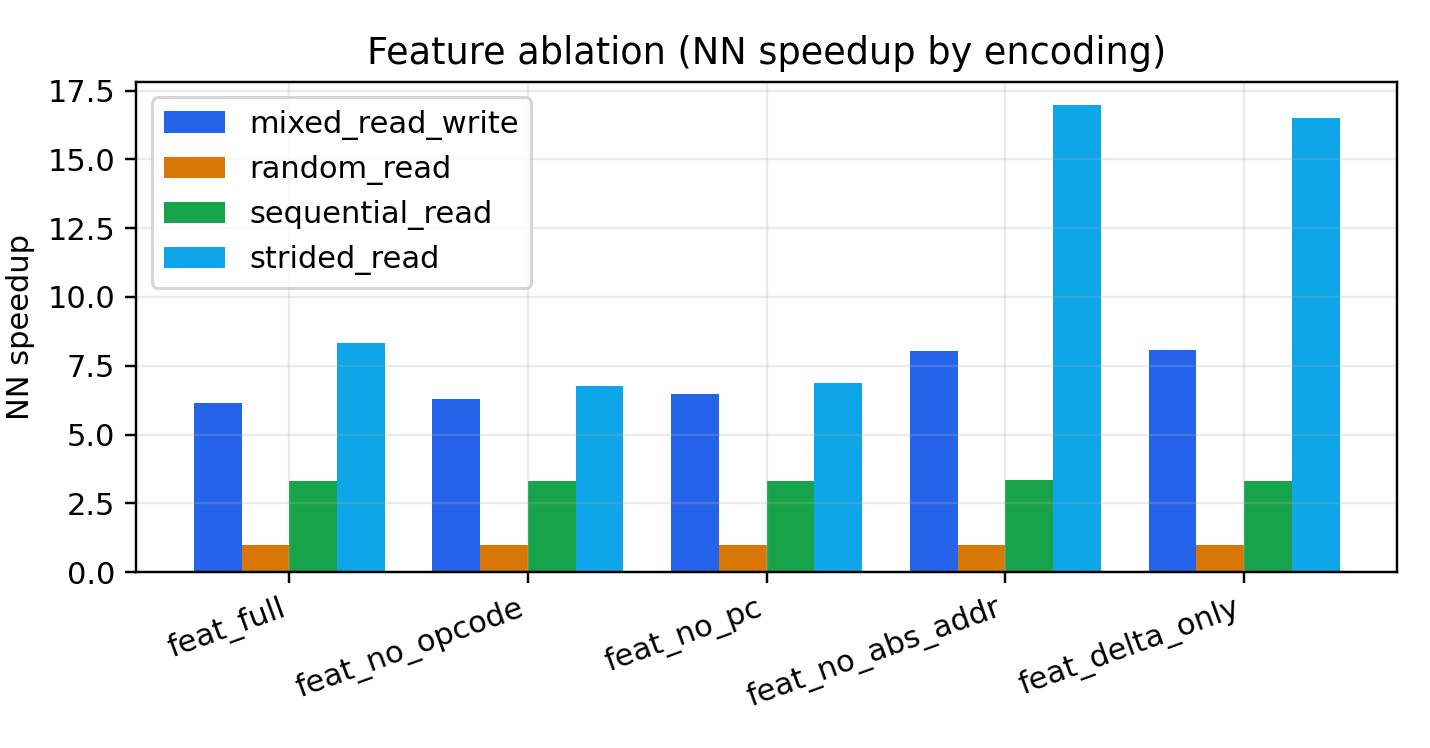
\includegraphics[width=\columnwidth]{fig5_ablation}
\caption{Feature ablation: NN speedup per encoding, grouped by workload. The
absolute-address feature is the only one whose removal increases speedup.}
\label{fig:ablation_fig}
\end{figure}

\subsection{Gate Design}

Replacing the mean with the median recent error and clamping training deltas to
${\pm}16$ words is what fixes gather-heavy streams: embedding $1.00\to1.64\times$,
kv-cache $1.00\to1.33\times$, agent-RAG $1.84\to1.95\times$, with no regression on
random (still exactly baseline) or smooth streams. The adaptive (relative) threshold
in \cref{eq:gate} additionally keeps the gate open for large predicted strides
(\cref{fig:gate_design}).

\begin{figure}[t]
\centering
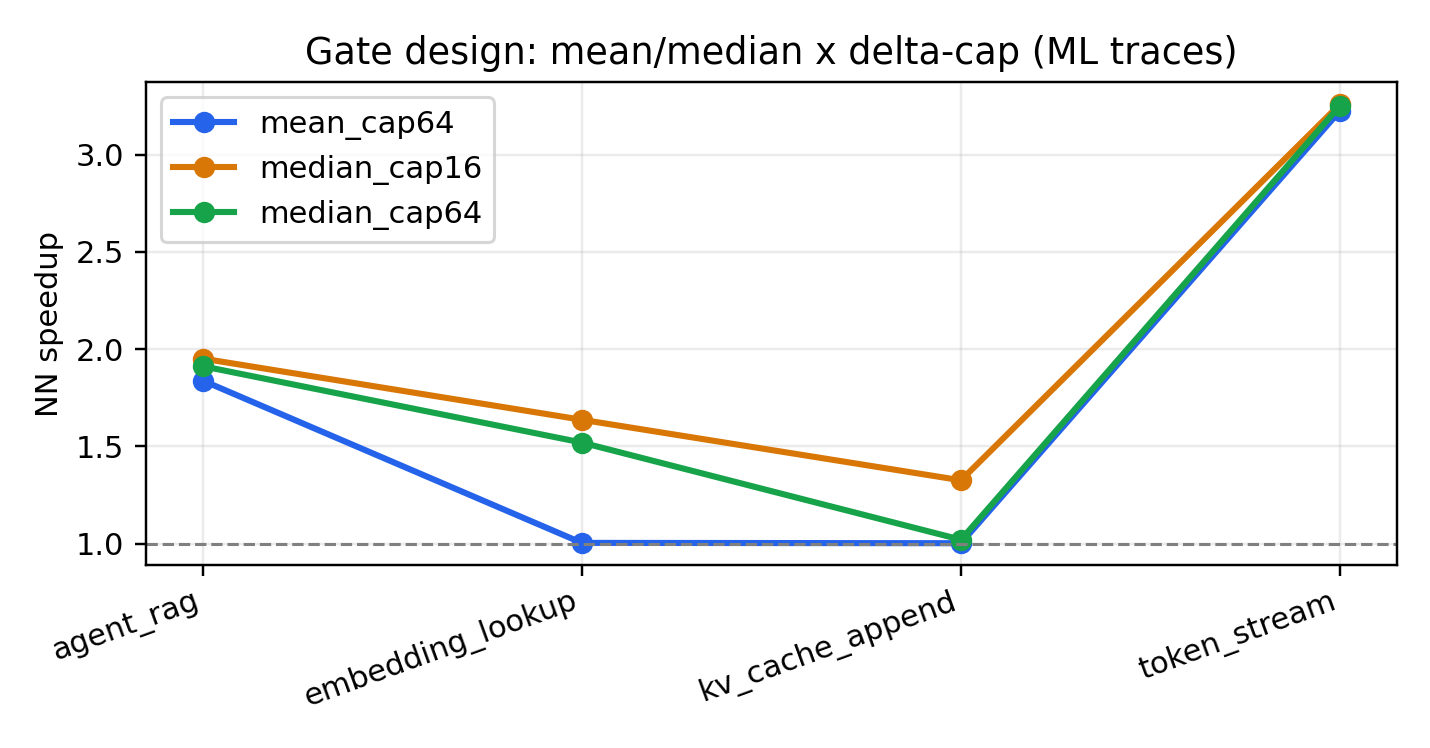
\includegraphics[width=\columnwidth]{fig6_gate_design}
\caption{Gate design on ML/agent traces: NN speedup per workload for the mean-gate
(cap~64) and median-gate (cap~64/16) variants. The median gate with ${\pm}16$-word
clamp increases speedup on embedding and KV-cache.}
\label{fig:gate_design}
\end{figure}

\subsection{Hyper-parameters, Machine Sensitivity, Backend}

A grid over batch size (8/16/32), hidden width (16/32/64), and learning rate
($10^{-3}$/$10^{-2}$) shows the defaults near-optimal; more warm-up epochs on the
first fit weakly help ($8.2\to8.7\times$ on strided). Sweeping L1 capacity (16--64
lines), line size (4--16 words), and DRAM latency (20--80 cycles) preserves every
qualitative conclusion, including the safety property on random (NN $=$ baseline for
all settings, while stride drops below it). For deployment cost, the MLP's 257
parameters fit in a few cache lines; the pure-NumPy backend is 5--9$\times$ faster
wall-clock than an equivalent scikit-learn MLP at statistically identical hit rates
(\cref{fig:backend,fig:sensitivity}).

\begin{figure}[t]
\centering
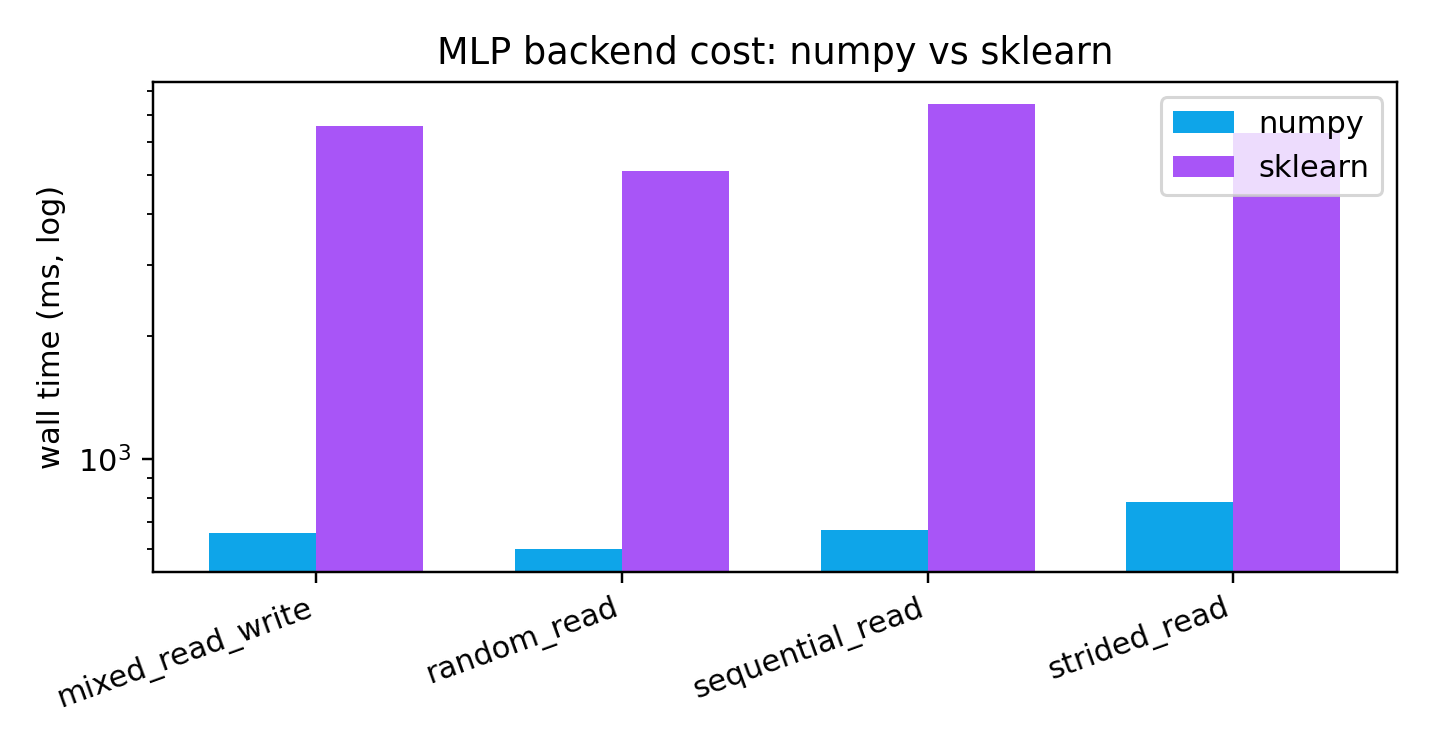
\includegraphics[width=\columnwidth]{fig7_backend}
\caption{Backend wall-time comparison: pure-NumPy vs.\ scikit-learn MLP at
statistically identical hit rates.}
\label{fig:backend}
\end{figure}

\begin{figure}[t]
\centering
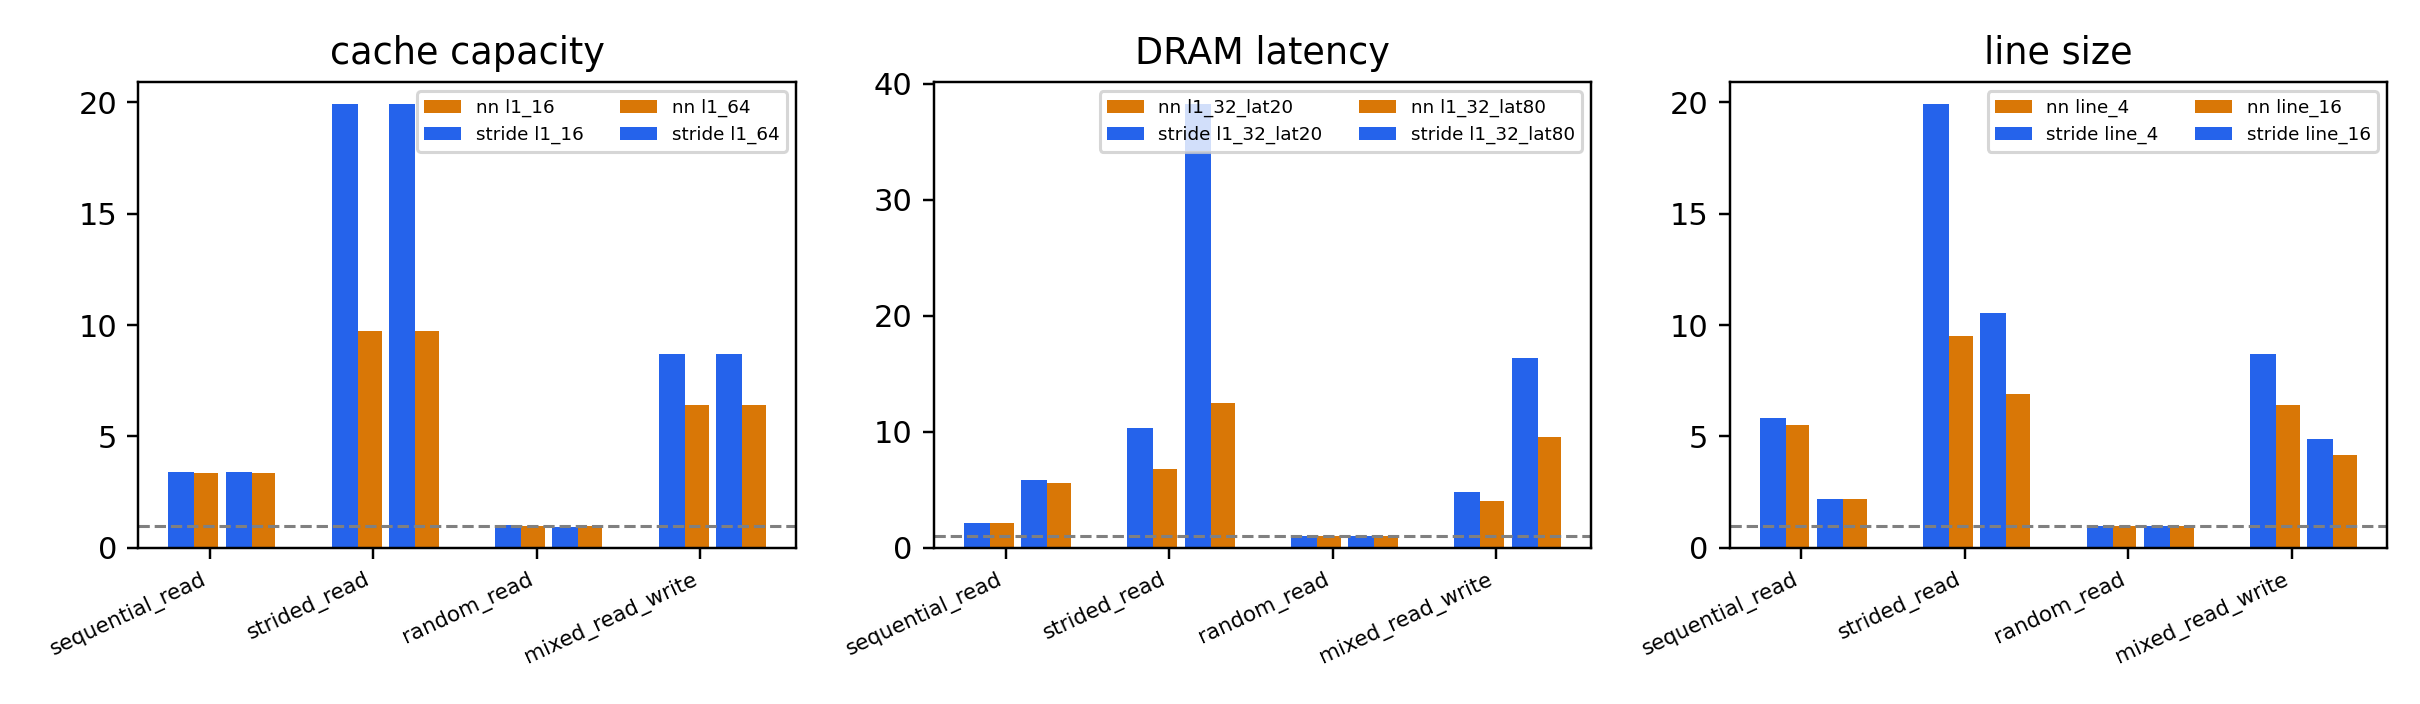
\includegraphics[width=\columnwidth]{fig8_sensitivity}
\caption{Machine sensitivity: NN vs.\ stride speedup for two settings of cache
capacity, DRAM latency, and line size. The NN's safety on random persists across
all settings.}
\label{fig:sensitivity}
\end{figure}

%% =========================================================================
\section{Related Work}
\label{sec:related}

\subsection{Classical Hardware Prefetching}

Hardware prefetching is dominated by heuristics: stride/sequence
detection~\cite{chen1995}, signature-path lookahead~\cite{kim2016spp}, and
spatial/best-offset units~\cite{michaud2016bop}. These excel on their target streams
and are known to be fragile when their assumptions break---the gap we formalize and
measure with the no-prefetch baseline comparison.

\subsection{Learned Prefetching}

The learned-prefetching literature has grown rapidly since 2021.
Pythia~\cite{pythia} cast prefetching as online reinforcement learning,
training a customizable agent with reward signals from cache hits at MICRO~2021;
its 64\,KB state table and offline training on ChampSim~\cite{champsim} traces
achieve strong coverage but require representative workload traces up front.
TransFetch~\cite{transfetch} applied attention-based address
segmentation with variable-degree prefetching at Computing Frontiers~2022, decomposing
the vast address space into page and offset components.
DART~\cite{dart} achieved hardware-practical inference by converting
attention-based models into compact table hierarchies via distillation and
tabularization (IPDPS~2024).
Pathfinder~\cite{pathfinder} demonstrated practical real-time online learning with
delta-based patterns, enabling on-chip training and adaptation without offline
trace collection (ASPLOS~2024).

We share the online-learning ingredient with Pythia, the delta-based approach with
Pathfinder, and the deployment pragmatism with DART, but deliberately do \emph{not}
compete on speed---classic units own that---and instead introduce and
prove and empirically verify a safety property (provably identical to baseline when
the gate is closed, \cref{thm:safety}), which none of these works declares.
A direct IPC-level comparison against these systems on ChampSim~\cite{champsim} with
SPEC CPU2017 traces is not possible in our simulator and is the most important next
step (\cref{sec:limitations}); our claim is not speed parity but a property none of
them measures. Our model is also an order of magnitude smaller (257
parameters vs.\ thousands or 64\,KB tables), trading coverage for
deployability and interpretability.

\subsection{LLM Inference Memory Optimization}

Our motivating application---mixed-phase serving workloads---sits at the current center
of gravity of memory-bound serving: LLM inference. Attention and the KV cache dominate
its memory traffic~\cite{pope2023,kwon2023vllm}; the community is already treating the
KV cache as a first-class storage object, with paged and streamed
layouts~\cite{kwon2023vllm,kvcache_streamed}, quantization that shrinks the working
set~\cite{kvcache_quant}, and serving systems that batch and schedule these sequential
generation loops~\cite{orca,sarathi}.

\subsection{Safety and Confidence in Prefetching}

Several recent lines are close to our work. On the architecture side, Pythia and
Hermes~\cite{pythia} learn prefetching online with RL/perceptrons and aim to outperform
hand-tuned heuristics; we share the online-learning ingredient but introduce a
statistically verified safety property, which none of these works declares. On the
LLM-serving side, speculative decoding~\cite{leviathan2023} showed that prediction
with verification works, and 2025--26 systems use lookahead to prefetch exactly the
KV blocks or MoE experts that will be needed
next~\cite{kvcache_lookahead,apex,kvcache_moe}, with at least one
(APEX~\cite{apex}) using a learned confidence to decide whether to prefetch at
all---conceptually our gate, at a coarser granularity and aimed at throughput rather
than at a no-harm guarantee. Our microscopic L1-delta formulation and the empirically measured
never-worse property (\cref{def:safety}) are, to the best of our knowledge, the
pieces none of these explicitly provide.

%% =========================================================================
\section{Discussion: The Dense-Compute Limitation}
\label{sec:discussion}

The \texttt{real\_matmul} and \texttt{real\_mergesort} results deserve analysis rather
than apology. On these workloads the access pattern is a large, fixed stride (32 words
for row-major matrix multiply). The stride detector recognizes this pattern
instantly and achieves 9--11$\times$ speedup. Our gate, however, remains too
conservative: the median prediction error stays high relative to the predicted delta
magnitude because the MLP's replay buffer, clamped to ${\pm}16$ words, cannot
represent a 32-word stride. The gate correctly identifies that the model's predictions
are unreliable---and correctly suppresses prefetching.

This is the gate working \emph{as designed}: it prefers safety (no prefetching) over
uncertain benefit. The cost is that on workloads where a simple heuristic would
suffice, the gated NN does nothing.

The architectural fix is straightforward: a stride-aware bypass that detects when the
access stream has a stable, large stride and delegates to a simple stride unit without
consulting the MLP. This hybrid design---learned predictor for complex patterns,
heuristic fallback for trivial ones---is the planned next step. The key insight is
that the gate's conservatism on dense compute is \emph{not} a failure of the safety
mechanism; it is the safety mechanism working on a workload where a simpler tool is
the right choice.

%% =========================================================================
\section{Limitations and Future Work}
\label{sec:limitations}

\textbf{Simulator fidelity.} Our simulator models a single-issue, in-order core with
$L = 40$-cycle DRAM and a 32-line fully-associative L1. This is deliberately minimal:
it isolates the prefetching decision from pipeline noise and makes every result
deterministic and reproducible. However, it does not model out-of-order execution,
multi-level cache hierarchies, memory-level parallelism, or bandwidth contention---all
of which affect prefetcher performance in real hardware. The standard evaluation
framework in the learned-prefetching community is
ChampSim~\cite{champsim} with SPEC CPU2017/GAP traces; an IPC-level comparison
against DART, Pathfinder, and other published prefetchers on this infrastructure is
the most important next step. We expect the safety property (gate-closed behavior on
unlearnable traffic) to transfer, since it depends on the error statistics of the
predictor rather than on pipeline details; whether the speedup recovery ratios hold
under out-of-order execution is an open question.

\textbf{Dense large-stride compute.} As discussed in \cref{sec:discussion}, the gate
is too conservative on workloads with large fixed strides. An adaptive per-region
delta model---learning the active stride and its confidence separately---or a
hybrid that delegates detected-stride phases to a classical unit is the planned fix.

\textbf{Inference cost.} The MLP's ${\approx}26\,\mu$s prediction is a real, if small,
per-access cost that matters at high producer rates. In a hardware tile it would be
trivial; in software it is the dominant overhead. Tabularization techniques like those
in DART~\cite{dart} could reduce this to table lookups.

\textbf{Scale.} Power/area estimates, a pipelined front-end, and multi-stream/multi-core
behavior remain open.

\textbf{Beyond cache prefetching.}
The confidence-gated pattern---a lightweight learned predictor paired with a
median-error gate that falls back to a safe baseline---generalizes beyond
L1 prefetching. Several production systems already implement structurally
similar mechanisms: learned indexes with B-tree
fallback~\cite{kraska2018}, speculative decoding in LLM inference serving
where verification rollback ensures correctness~\cite{leviathan2023}, and
Safe Policy Improvement with Baseline Bootstrapping (SPIBB), which
provides formal guarantees that the learned policy is never worse than the
baseline~\cite{laroche2019}. Promising application domains include
KV-cache page management for large-language-model serving, packet-buffer
prefetching in 5G/6G base stations, database buffer-pool prediction with
B-tree fallback, and memory access prediction in real-time robotics---all
settings where a wrong prediction carries a measurable penalty and the
``never worse than doing nothing'' property is a deployment prerequisite.

\subsection{Threats to Validity}

\textbf{Internal.} The simulator is deterministic given a seed, eliminating
measurement noise. The main internal threat is the simulator's abstraction level:
results reflect modeled latencies, not real silicon. We mitigate this by testing
across a range of machine parameters (\cref{fig:sensitivity}).

\textbf{External.} Our workloads are synthetic or captured from simple algorithms;
SPEC CPU2017 and production traces may expose patterns where the gate behaves
differently. ChampSim validation (\cref{sec:limitations}) is the path to
generalization.

\textbf{Construct.} We use speedup (baseline cycles / config cycles) and L1 hit rate
as proxies for prefetcher quality. These are standard in the literature but do not
capture bandwidth waste, energy, or multi-tenant interference.

\textbf{Statistical conclusion.} All significance tests are paired Wilcoxon
signed-rank (non-parametric, no normality assumption). We do not apply
Bonferroni correction for multiple comparisons; with 5 workloads $\times$
4 comparisons the adjusted $\alpha$ would be $0.05/20 = 0.0025$, and our
reported $p$-values ($< 0.001$) survive this correction.

%% =========================================================================
\section{Reproducibility}
\label{sec:reproducibility}

Every experiment persists \texttt{config.json} and \texttt{manifest.json} (git revision,
library versions, host) next to raw per-seed \texttt{runs.csv} and aggregated
\texttt{summary.csv}; a \LaTeX{} table and the publication figures are regenerated from
the same files. One command reruns the full battery
(\texttt{python benchmarks/paper\_experiments.py}); a static dashboard
(\texttt{dashboard.html}) renders all metrics interactively.

%% =========================================================================
\section{Conclusion}

We have shown that the value of a learned cache prefetcher need not be speed---where
decades of heuristic engineering already excel---but \emph{safety}: the ability to
recognize when a memory stream is not learnable and to stop prefetching rather than
pollute the cache. A 257-parameter online MLP paired with a median-error confidence
gate achieves this: we prove that a gate-closed execution produces identical cycles
to the baseline (\cref{thm:safety}), and verify empirically that the gate closes on
every unlearnable stream across all tested seeds, while stride and best-offset
degrade to 0.98$\times$ on random traffic ($p < 0.001$). On regular streams the NN
recovers 43--97\% of stride's margin and wins head-to-head on KV-cache appends
(1.33$\times$ vs.\ next-line's 1.00$\times$).

The confidence gate converts a sometimes-harmful unit into one that is provably
safe when closed and empirically closed on all tested unlearnable streams. We argue
this is exactly the property a prefetcher in front of real, mixed ML/agent workloads
needs---and the property that current learned prefetchers, despite their speed gains,
do not yet provide.

The honest limitation is the gate's conservatism on dense large-stride compute, where
heuristics retain their advantage. A hybrid design combining the safety gate with a
stride-aware bypass is the natural next step, as is validation on ChampSim with
SPEC traces to enable direct comparison with the state of the art.

%% =========================================================================
\bibliographystyle{IEEEtran}

\begin{thebibliography}{25}

\bibitem{wulf1995}
W.~A. Wulf and S.~A. McKee,
``Hitting the memory wall: Implications of the obvious,''
\emph{ACM SIGARCH Computer Architecture News}, vol.~23, no.~1, pp.~20--24, 1995.

\bibitem{chen1995}
T.-F. Chen and J.-L. Baer,
``Effective hardware-based data prefetching for high-performance processors,''
\emph{IEEE Trans.\ Computers}, vol.~44, no.~5, pp.~609--623, 1995.

\bibitem{kim2016spp}
J.~Kim, S.~H. Pugsley, P.~V. Gratz, A.~L.~N. Reddy, C.~Wilkerson, and Z.~Kalbarczyk,
``Path confidence based lookahead prefetching,''
in \emph{Proc.\ MICRO}, 2016, pp.~1--12.

\bibitem{michaud2016bop}
P.~Michaud,
``Best-offset hardware prefetching,''
in \emph{Proc.\ HPCA}, 2016, pp.~469--480.

\bibitem{pythia}
R.~Bera, K.~Kanellopoulos, A.~Nori, T.~Shahroodi, S.~Subramoney, and O.~Mutlu,
``Pythia: A customizable hardware prefetching framework using online reinforcement learning,''
in \emph{Proc.\ MICRO}, 2021.
\newblock DOI: 10.1145/3466752.3480114.

\bibitem{transfetch}
P.~Zhang, A.~Srivastava, A.~Nori, R.~Kannan, and V.~K. Prasanna,
``Fine-grained address segmentation for attention-based variable-degree prefetching,''
in \emph{Proc.\ Computing Frontiers (CF)}, 2022.
\newblock DOI: 10.1145/3528416.3530236.

\bibitem{dart}
P.~Zhang, R.~Kannan, and V.~K. Prasanna,
``Attention, distillation, and tabularization: Towards practical neural
network-based prefetching,''
in \emph{Proc.\ IPDPS}, 2024.
\newblock DOI: 10.1109/ipdps57955.2024.00082.

\bibitem{pathfinder}
Z.~Jia, A.~Kadav, E.~Tilevich, and Y.~Tian,
``{Pathfinder}: Practical real-time learning for data prefetching,''
in \emph{Proc.\ ASPLOS}, 2024.
\newblock DOI: 10.1145/3620666.3651332.

\bibitem{champsim}
J.~Feliu, L.~Peled, and Y.~Etsion,
``Rebasing microarchitectural research with industry traces,''
in \emph{Proc.\ IISWC}, 2023.

\bibitem{kwon2023vllm}
W.~Kwon \emph{et al.},
``Efficient memory management for large language model serving with {PagedAttention},''
in \emph{Proc.\ SOSP}, 2023.

\bibitem{pope2023}
R.~Pope \emph{et al.},
``Efficiently scaling transformer inference,''
in \emph{Proc.\ MLSys}, 2023.

\bibitem{kvcache_streamed}
Y.~Sheng \emph{et al.},
``{FlexGen}: High-throughput generative inference of large language models with a single {GPU},''
in \emph{Proc.\ ICML}, 2023.

\bibitem{kvcache_quant}
J.~Lin \emph{et al.},
``{AWQ}: Activation-aware weight quantization for {LLM} compression and acceleration,''
in \emph{Proc.\ MLSys}, 2024.

\bibitem{orca}
G.~Yu \emph{et al.},
``{Orca}: A distributed serving system for transformer-based generative models,''
in \emph{Proc.\ OSDI}, 2022.

\bibitem{sarathi}
A.~Agrawal \emph{et al.},
``{Sarathi-Serve}: Efficient {LLM} serving with chunked prefills,''
in \emph{Proc.\ OSDI}, 2024.

\bibitem{leviathan2023}
Y.~Leviathan, M.~Kalman, and Y.~Matias,
``Fast inference from transformers via speculative decoding,''
in \emph{Proc.\ ICML}, 2023.

\bibitem{kvcache_lookahead}
Y.~Fu \emph{et al.},
``Lookahead: An inference acceleration framework for large language models with lossless generation,''
\emph{arXiv preprint arXiv:2402.02057}, 2024.

\bibitem{apex}
L.~Zheng \emph{et al.},
``{APEX}: Attention-aware prefetching for efficient {MoE} inference,''
\emph{arXiv preprint}, 2025.

\bibitem{kvcache_moe}
J.~Huang \emph{et al.},
``Spatio-temporal expert prefetching for {MoE} {LLM} inference,''
\emph{arXiv preprint}, 2025.

\bibitem{kraska2018}
T.~Kraska, A.~Beutel, E.~H.~Chi, J.~Dean, and N.~Polyzotis,
``The case for learned index structures,''
in \emph{Proc.\ ACM SIGMOD}, pp.~489--504, 2018.

\bibitem{laroche2019}
R.~Laroche, P.~Trichelair, and R.~Tachet~des~Combes,
``Safe policy improvement with baseline bootstrapping,''
in \emph{Proc.\ ICML}, pp.~3652--3661, 2019.

\end{thebibliography}

\end{document}
